%; whizzy chapter
% -initex iniptex -latex platex -format platex -bibtex jbibtex -fmt fmt
% $B0J>e(B whizzytex $B$r;HMQ$9$k>l9g$N@_Dj!#(B


%     Tokyo Debian Meeting resources
%     Copyright (C) 2010 Junichi Uekawa

%     This program is free software; you can redistribute it and/or modify
%     it under the terms of the GNU General Public License as published by
%     the Free Software Foundation; either version 2 of the License, or
%     (at your option) any later version.

%     This program is distributed in the hope that it will be useful,
%     but WITHOUT ANY WARRANTY; without even the implied warranty of
%     MERCHANTABILITY or FITNESS FOR A PARTICULAR PURPOSE.  See the
%     GNU General Public License for more details.

%     You should have received a copy of the GNU General Public License
%     along with this program; if not, write to the Free Software
%     Foundation, Inc., 51 Franklin St, Fifth Floor, Boston, MA  02110-1301 USA

%  preview (shell-command (concat "evince " (replace-regexp-in-string "tex$" "pdf"(buffer-file-name)) "&"))
% $B2hA|%U%!%$%k$r=hM}$9$k$?$a$K$O(Bebb$B$rMxMQ$7$F(Bboundingbox$B$r:n@.!#(B
%(shell-command "cd image201002; ebb *.png")

%%$B$3$3$+$i%X%C%@3+;O!#(B

\documentclass[mingoth,a4paper]{jsarticle}
\usepackage{monthlyreport}
\usepackage{wrapfig}

% $BF|IU$rDj5A$9$k!"Kh7nJQ$o$j$^$9!#(B
\newcommand{\debmtgyear}{2010}
\newcommand{\debmtgmonth}{2}
\newcommand{\debmtgdate}{20,21}
\newcommand{\debmtgnumber}{61}

\begin{document}

\begin{titlepage}
\thispagestyle{empty}

% $B%?%$%H%k%Z!<%8(B:$BJT=8I,MW$JItJ,$O:G=i$N%^%/%m$KHt$P$9$3$H(B

\vspace*{-2cm}
$BBh(B\debmtgnumber{}$B2s(B $BEl5~%(%j%"(B Debian $BJY6/2q;qNA(B

\hspace*{-2.4cm}
\includegraphics[width=210mm]{image200801/2008title.eps}\\
\hfill{}\debmtgyear{}$BG/(B\debmtgmonth{}$B7n(B\debmtgdate{}$BF|(B

\end{titlepage}


\dancersection{Introduction}{$B>e@n(B $B=c0l(B}

\begin{multicols}{2}
 
 
 $B:#7n$N(BDebian$BJY6/2q$X$h$&$3$=!#$3$l$+$i(BDebian$B$N@$3&$K$"$7$rF'$_F~$l$k$H(B
 $B$$$&J}$b!"$9$G$K$I$C$W$j$H$D$+$C$F$$$k$H$$$&J}$b!"7n$K0l2s(BDebian$B$K$D$$(B
 $B$F8l$j$^$;$s$+!)(B

 Debian$BJY6/2q$NL\E*$O2<5-$G$9!#(B

 \begin{itemize}
 \item \underline{Debian Developer} ($B3+H/<T(B)$B$N0i@.!#(B
 \item $BF|K\8l$G$N!V(B\underline{$B3+H/$K4X$9$k>pJs(B}$B!W$r@0M}$7$F$^$H$a!"%"%C%W%G!<%H$9$k!#(B
 \item \underline{$B>l(B}$B$NDs6!!#(B
 \begin{itemize}
  \item $BIaCJ$P$i$P$i$J>l=j$K$$$k?M!9$,(B face-to-face $B$G=P2q$($k>l$rDs6!(B
	$B$9$k!#(B
  \item Debian $B$N$?$a$K$J$k$3$H$r8l$k>l$rDs6!$9$k!#(B
  \item Debian$B$K$D$$$F8l$k>l$rDs6!$9$k!#(B
 \end{itemize}
 \end{itemize}		

 Debian$B$NJY6/2q$H$$$&$3$H$G5f6KE*$K$O;22C<TA40w$,(BDebian Package$B$r$,$j$,$j(B
 $B$H:n$k%9!<%Q!<%O%C%+!<$K$J$C$?;Q$rLQA[$7$F$$$^$9!#>pJs$N6&M-!&3hMQ$rDL$7(B
 $B$F(B Debian$B$N:#8e$NG=F0E*$JE83+$X$NEZBf$H$7$F!"!V>l!W$H$7$F$N6u4V$rDs6!$9(B
 $B$k$N$,L\E*$G$9!#(B

\end{multicols}

\newpage

\begin{minipage}[b]{0.2\hsize}
 \definecolor{titleback}{gray}{0.9}
 \colorbox{titleback}{\rotatebox{90}{\fontsize{80}{80} {\gt $B%G%S%"%sJY6/2q(B} }}
\end{minipage}
\begin{minipage}[b]{0.8\hsize}
\hrule
\vspace{2mm}
\hrule
\tableofcontents
\vspace{2mm}
\hrule
\end{minipage}

\dancersection{$B;vA02]Bj(B}{$B>e@n(B $B=c0l(B}

$B:#2s$N;vA02]Bj$O0J2<$G$9(B:

\begin{enumerate}
 \item $B;vA02]Bj$NFbMF(B
\end{enumerate}

$B$3$N2]Bj$KBP$7$FDs=P$$$?$@$$$?FbMF$O0J2<$G$9!#(B

\begin{prework}{ �����ϥ� }
\begin{enumerate}
\item �ϻϼԤ� Ian ����Ȥ��κ� Debra �����̾������̿̾���줿�� 
\item ���äѤ����ꤹ���ơ�������ˤ����ޤ�ʤ���
\item ���֤���ͳ�ϡ���ʬ�����ޤΤ��㤯�����餫�ʤ���
\end{enumerate}
\end{prework}
\begin{prework}{ emasaka }
\begin{enumerate}
\setcounter{enumi}{2}
\item �Ȥˤ�����������Υѥå��������鹽��������ǡ����뤤��ɬ�פ˱�����
      �ѥå��������ɲä��ơ��ʤ����Ĥ������ٰ¿����ơ����Ӥ˹�ä�������
      ����Ȥ������
\end{enumerate}
\end{prework}
\begin{prework}{ henrich }
\begin{enumerate}
\item dis���ʤ���⤬��Ф�򵤤ʥץ��������ȤǤ���
\item �ץ��������ȥ꡼�����γ�ư�����β����Ƥ�Ρ���
\item �ֱ郎���ä�����פǤ� :)
\end{enumerate}
\end{prework}
\begin{prework}{ mkouhei }
\begin{enumerate}
\setcounter{enumi}{2}
\item ʣ���Υ������ƥ�����Υޥ���򡢤��ΰ㤤�򵤤ˤ��������ѤǤ���ѥ�
      �����������ƥब���������뤿��Ǥ����Ȥ��Ϥ᤿���ä����Ǥ⤢��ޤ���
      �����ǻȤäƤ���Τ����Ǥ�5����Ǥ���
\end{enumerate}
\end{prework}
\begin{prework}{ ����(yy\_y\_ja\_jp) }
\begin{enumerate}
\setcounter{enumi}{2}
\item DFSG�����뤫�顥\&�ѥå������󥰥����ƥबͥ��Ƥ��뤫�顥�Ǥ��͡�
\end{enumerate}
\end{prework}
\begin{prework}{ ������ }
\begin{enumerate}
\setcounter{enumi}{2}
\item ������������ۤΥѥå��������������ƥ�˽в�ä��Ȼפäư��衢���äȻȤäƤޤ���
\end{enumerate}
\end{prework}


\dancersection{$B:G6a$N(BDebian$B4XO"$N%_!<%F%#%s%0Js9p(B}{$B>e@n=c0l(B}
\subsection{$BEl5~%(%j%"(BDebian$BJY6/2q(B60$B2sL\Js9p(B}
% (query-replace-regexp "<.*?>" "")
% (query-replace-regexp "^[	 ]\+" "")

$BA02s$N(B BSP $B$N3+:EJs9p(B


% =======================================================================
\dancersection{$B4X?t7?=hM}7O$NOC(B}{$BF|HfLn7<(B}
\index{functional programming}
% =======================================================================

\subsection{hoge}
\subsubsection{subhoge}

% =======================================================================
\dancersection{$B$J$<(B Debian $B$J$N$+(B}{$B$d$^$M$R$G$-(B}
\index{why debian}
% =======================================================================

\subsection{hoge}
\subsubsection{subhoge}

% =======================================================================
\dancersection{$B%V!<%HJ}K!$,JQ$o$k$h(B}{$B$^$($@$3$&$X$$(B}
\index{upstart}
% =======================================================================

\subsection{Squeeze $B$+$i%V!<%HJ}K!$,JQ$o$k(B}
Debian $B$N%V!<%H$N;EAH$_$K$O!"(BSystem-V $B7O(B Unix $B$G$OEAE}E*$J(B init
(sysvinit) $B$,;H$o$l$F$$$^$9!#(BDebian $B$N<!4|0BDjHG(B6.0 ($B%3!<%I%M!<%`(B
Squeeze) $B$+$i!"$3$l$,(B upstart $B$KJQ$o$kM=Dj$G$9!#:#G/$N(B 3 $B7n$K%U%j!<%:M=(B
$BDj!"(B8$B7n$K%j%j!<%9M=Dj$N(BSqueeze $B$G$NM==,$N0UL#$r9~$a$F!":#2s$O$3$N(B
upstart $B$KJQ$o$k$3$H$K$J$C$?GX7J!"(Binit $B$H$NHf3S$r4^$a$?(B upstart $B$N;EAH$_!"(B
$B<B:]$K@Z$jBX$(J}K!$K$D$$$F@bL@$7$^$9!#(B

\subsubsection{$BGX7J(B}

upstart $B$O!"(BDebian $B$r%Y!<%9$H$7$?%G%#%9%H%j%S%e!<%7%g%s$G$"$k!"(BUbuntu $BFH(B
$B<+$K(B sysvinit $B$N8e7Q$N;EAH$_$H$7$F3+H/$5$l$^$7$?!#85!9(B sysvinit $B$OEAE}E*(B
$B$G0BDj$7$?;EAH$_$G$O$"$j$^$9$,!"8=:_;H$o$l$F$$$k%O!<%I%&%'%"$G;H$&$K$O5!(B
$BG=LL!"@-G=LL$+$iLdBj$,=P$F$-$F$$$^$9!#$=$3$G!"(Bsysvinit $B$N8e7Q$N;EAH$_$H(B
$B$7$F!"(Bupstart $B0J30$K$bJ#?t$N%V!<%H%W%m%;%9$N;EAH$_$,3+H/$5$l$F$$$^$9!#$7(B
$B$+$7!"(BUbuntu $B0J30$K$b(B Fedora $B$d(B ???, ??? $B$H$$$C$?<gMW$J%G%#%9%H%j%S%e!<(B
$B%7%g%s$G$O(B upstart $B$,:NMQ$5$l!"(BDebian $B$G$b(B Squeeze $B$+$i:NMQ$5$l$k(B($BM=Dj(B)
$B$H$$$&$3$H$b$"$j!"(Bsysvinit $B$N8e7Q$O(B upstart $B$KMn$ACe$/$@$m$&$H8+$i$l$F$$(B
$B$^$9!#(B

\subsubsection{$B$=$b$=$b(B init $B$C$F2?$h!)(B}

upstart $B$NOC$r$9$kA0$K!"(Binit $B$C$F2?!)$H$$$&?M8~$1$K$^$:@bL@$7$^$7$g$&!#(B
init $B$O:#99@bL@$7$J$/$F$bCN$C$H$k$,$J!"$H$$$&FI<T$O!"@h$KFI$_?J$a$F$/$@(B
$B$5$$!#(B

init $B$O(B Unix/Linux $B%7%9%F%`$K$*$$$F!"%+!<%M%k$,%V!<%H$7$?8e!"%f!<%6%W%m(B
$B%0%i%`$,5/F0$9$k$?$a$N;EAH$_$G$9!#Nc$($P!"$"$J$?$N;H$C$F$$$k%N!<%H(B PC $B$d(B
$B%5!<%P$KF~$C$F$$$k(B Debian $B%7%9%F%`$G$b$3$N;EAH$_$,I,$:F~$C$F$$$^$9!#%^%7(B
$B%s$KEE8;$rF~$l$F$+$i!"%m%0%$%s2hLL$,I=<($5$l$k$^$G$NN.$l$OBg$^$+$K$O<!$N(B
$B$h$&$K$J$j$^$9!#(B

\begin{figure}[H]
\begin{center}
\includegraphics[height=0.8\hsize]{image201002/sysvinit.eps}
\end{center}
\end{figure}

init $B%W%m%;%9$,5/F0$9$k$H!"(Binit $B$O(B /etc/inittab $B$NFbMF$K=>$C$F!"%W%m%;%9(B
$B$N$r@8@.$dDd;_$r9T$$$^$9!#(Binittab $B$N=q<0$O<!$N$h$&$K$J$j$^$9!#(B

\begin{commandline}
id:runlevels:action:process
\end{commandline}


$B%W%m%;%9$N@8@.$K4X$o$kItJ,$K$O0J2<$N$h$&$J$b$N$,$"$j$^$9!#(B

\begin{commandline}
si::sysinit:/etc/init.d/rcS

l1:1:wait:/etc/init.d/rc 1
l2:2:wait:/etc/init.d/rc 2
l3:3:wait:/etc/init.d/rc 3
l4:4:wait:/etc/init.d/rc 4
l5:5:wait:/etc/init.d/rc 5
\end{commandline}

$B0l9TL\$K%i%s%l%Y%k$N;XDj$,L5$$$N$O!"(Baction $B$K(B sysinit $B$,;XDj$5$l$F$$$k$?(B
$B$a$G$9!#$3$l$O%9%F%`%V!<%HCf$K<B9T$5$l!"B>$N%V!<%HMQ$N(B action $B$h$j$bM%@h(B
$B$7$F<B9T$5$l$^$9!#(B/etc/init.d/rcS $B$G$O(B

\begin{commandline}
exec /etc/init.d/rc S
\end{commandline}

$B$@$1$,<B9T$5$l$^$9!#$3$l$O(B /etc/init.d/rc $B$G$N%V!<%HMQ$NJQ?t$r@_Dj$7$^$9!#(B
$B$3$N8e!">e5-$N(B rc $B%9%/%j%W%H$KBP$7!"5/F0;~$K;XDj$9$k%i%s%l%Y%k$r(B $B0z?t$H(B
$B$7$F<B9T$5$l$^$9$,!"(BDebian $B$G$N%G%U%)%k%H$O!"%i%s%l%Y%k(B 2$B$G5/F0$5$l$^$9!#(B

\begin{commandline}
id:2:initdefault:
\end{commandline}

$B$J$N$G!"<B:]$K$O2<5-$,<B9T$5$l$^$9!#(B

\begin{commandline}
l2:2:wait:/etc/init.d/rc 2
\end{commandline}

$B$3$l$K$h$j(B /etc/rc2.d $B0J2<$N%U%!%$%kL>$,(B \textbf{S??} $B$G;O$^$k%9%/%j%W%H(B
$B$,(B ``??''$B$NFs7e$N?t;z$NItJ,$,(B''\textbf{$B>:=g$G$"$k$h$&$K0l$D$:$D<B9T(B}''$B$5(B
$B$l$^$9!#F1$8%l%Y%k$N%9%/%j%W%H$OJB9T$7$F<B9T$5$l$^$9$,!"$3$l$,5/F0$,CY$/(B
$B$J$k860x$N0l$D$K$J$C$F$$$^$9!#(B

\begin{commandline}
# Now run the START scripts for this runlevel.
# Run all scripts with the same level in parallel
CURLEVEL=""
for s in /etc/rc$runlevel.d/S*
do
        # Extract order value from symlink
        level=${s#/etc/rc$runlevel.d/S}
        level=${level%%[a-zA-Z]*}
        if [ "$level" = "$CURLEVEL" ]
        then
                continue
        fi
        CURLEVEL=$level
        SCRIPTS=""
        for i in /etc/rc$runlevel.d/S$level*
        do
                [ ! -f $i ] && continue

                suffix=${i#/etc/rc$runlevel.d/S[0-9][0-9]}
                if [ "$previous" != N ]
                then
                        #
                        # Find start script in previous runlevel and
                        # stop script in this runlevel.
                        #
                        stop=/etc/rc$runlevel.d/K[0-9][0-9]$suffix
                        previous_start=/etc/rc$previous.d/S[0-9][0-9]$suffix
                        #
                        # If there is a start script in the previous level
                        # and _no_ stop script in this level, we don't
                        # have to re-start the service.
                        #
                        if [ start = "$ACTION" ] ; then
                                [ -f $previous_start ] && [ ! -f $stop ] && continue
                        else
                                # Workaround for the special
                                # handling of runlevels 0 and 6.
                                previous_stop=/etc/rc$previous.d/K[0-9][0-9]$suffix
                                #
                                # If there is a stop script in the previous level
                                # and _no_ start script there, we don't
                                # have to re-stop the service.
                                #
                                [ -f $previous_stop ] && [ ! -f $previous_start ] && continue
                        fi

                fi
                SCRIPTS="$SCRIPTS $i"
                if is_splash_stop_scripts "$suffix" ; then
                        $debug splash_stop || true
                fi
        done
        startup $ACTION $SCRIPTS
done
\end{commandline}

$B$J$*!"A0=R$N$H$*$j!"(BDebian $B$G$O%G%U%)%k%H$N%i%s%l%Y%k$O(B 2 $B$G$9!#(BDebian
$B$G$O(B 2$B$+$i(B5 $B$N%i%s%l%Y%k$O4pK\E*$K$OF1$8$G!"%i%s%l%Y%k(B 2 $B$7$+;H$$$^$;$s!#(B
$BB>$N%G%#%9%H%j%S%e!<%7%g%s$N$h$&$K!"%i%s%l%Y%k(B 3 $B$O%F%-%9%H%b!<%I!"%i%s(B
$B%l%Y%k(B 5 $B$O(B X Window System $B$,N)$A>e$,$k!"$H$$$&@Z$jBX$($O$7$^$;$s!#$3$l(B
$B$O(B Debian $B$G$O!"%$%s%9%H!<%k$5$l$F$$$k%Q%C%1!<%8$H$$$&$N$O!"%f!<%6$,I,MW(B
$B$@$+$i%$%s%9%H!<%k$7$F$$$k$N$G$"$k!"$H$$$&9M$($K4p$E$-!"%$%s%9%H!<%k$7$?(B
$B%Q%C%1!<%8$OA4$F:G=i$+$i;H$($k$h$&$K$J$C$F$*$j!"%5!<%S%9$G$"$l$P>o;~2TF0(B
$B$9$k$h$&$K$J$C$F$$$^$9!#$?$@$7!":G6a$G$O(B $B%$%s%9%H!<%k$7$F$"$C$F$b%7%9%F(B
$B%`%V!<%H;~$K$O5/F0$;$:!"%f!<%6(B\footnote{$B$3$3$G$$$&%f!<%6$H$O!"%7%9%F%`4I(B
$BM}<T$KBP$9$k%(%s%I%f!<%6!"$G$O$J$/(B Debian $B%7%9%F%`$rMxMQ$9$k(B Debian $B%f!<(B
$B%6$N$3$H$r;X$7$F$$$^$9!#(B}$B$,G$0U$N;~$K5/F0=PMh$k$h$&$K(B /etc/default/ $B0J2<(B
$B$N@_Dj%U%!%$%k$G@)8f$G$-$k$h$&$K$J$C$F$$$k$b$N$b$"$j$^$9!#(B


$B5/F0%9%/%j%W%H$N5/F00J30$K$O!"%i%s%l%Y%k(B 2 $B$+$i(B 5 $B$^$?$O!"(B2 $B$+(B 3 $B$N;~$K(B
$B$O%3%s%=!<%k$+$i(B getty $B$,<B9T$5$l$^$9!#(Baction $B$,(B \texttt{respawn} $B$H$J$C(B
$B$F$$$^$9$,!"$3$l$O(B getty $B%W%m%0%i%`$,=*N;$7$?$i!"(Binit $B$,:F5/F0$5$;$k$?$a(B
$B$N;X<($G$9!#$"$k%f!<%6$,%3%s%=!<%k$+$i%m%0%$%s$7$?%;%C%7%g%s$r!"%m%0%"%&(B
$B%H$9$k$H(B getty $B$O=*N;$7$^$9$,!"(Binit $B$K$h$j:F$S(B $B%m%0%$%s2hLL$GBT$A<u$1$k(B
$B$3$H$,$G$-$k!"$H$$$&$o$1$G$9!#(B

\begin{commandline}
1:2345:respawn:/sbin/getty 38400 tty1
2:23:respawn:/sbin/getty 38400 tty2
3:23:respawn:/sbin/getty 38400 tty3
4:23:respawn:/sbin/getty 38400 tty4
5:23:respawn:/sbin/getty 38400 tty5
6:23:respawn:/sbin/getty 38400 tty6
\end{commandline}

$BB>$N(B init $B$NLr3d$H$7$F$O!"%7%9%F%`Dd;_;~$N%W%m%;%9$NDd;_$K$b4X$o$C$F$$$^(B
$B$9!#(B

\subsection{upstart $B$H$O(B}

\begin{commandline}

upstart
=======

Upstart is a replacement for the traditional sysvinit package, and
runs as process #1.  While it is eventually intended to be used to
create a completely event-driven boot process, we are currently
only using it to emulate the original sysvinit behaviour.

This gives us the maximum amount of testing of the code and concepts
behind it, while retaining the ability to fallback to sysvinit should
things not work out.

This file documents how to do a few common operations with the new
system.


Where are initscripts installed?
--------------------------------

This has not changed, they are installed in /etc/init.d.  See
/etc/init.d/README.


How are initscripts started and stopped?
----------------------------------------

This has not changed, symlinks are made from the initscript in the
/etc/init.d directory to the /etc/rc?.d directories.  See
/etc/init.d/README and /etc/rc?.d/README.


What order are initscripts started and stopped in?
--------------------------------------------------

This has not changed, the symlinks are named SNNname or KNNname, where
NN is a number from 00 to 99.  The K scripts are run first in
numerical order, followed by the S scripts in numerical order.


How do I find the current/previous runlevel?
--------------------------------------------

This has not changed, use the "runlevel" command.  See runlevel(8).


How do I change the runlevel?
-----------------------------

This has not changed, use the "telinit" command or just invoke "init"
directly.  See telinit(8).


How do I change the default runlevel?
-------------------------------------

Edit the /etc/inittab file.  Locate, or write, the following line:

    id:N:initdefault:

Where N is the default runlevel, change this to match.


How do I shutdown the machine?
------------------------------

This has not changed, use the "shutdown" command provided by the
upstart package; you may also use the "reboot"/"halt"/"poweroff"
commands as a short-cut.  See shutdown(8) and reboot(8).

You can also press Control-Alt-Delete on a console to reboot the
machine.


How do I change the behaviour of Control-Alt-Delete?
----------------------------------------------------

Edit the /etc/init/control-alt-delete.conf file, the line beginning
"exec" is what upstart will run when this key combination is pressed.

To not do anything, you can simply delete this file.


How do I enter single-user mode?
--------------------------------

This hasn't changed, choose the "(recovery mode)" option from GRUB;
add "-s", "S" or "single" to the kernel command-line; or from a
running machine, run "telinit 1" or "shutdown now".


How do I reduce the number of gettys?
-------------------------------------

Also see "How do I change which runlevels gettys are run in?"

In /etc/init there is a file named ttyN.conf for each getty that will be
started, where N is numbered 1 to 6.  Remove any that you do not
want.

This will not take immediate effect, however you can run "stop ttyN"
to stop one that is running.


How do I change getty parameters?
---------------------------------

In /etc/init there is a file named ttyN.conf for each getty that will be
started, where N is numbered 1 to 6.  Edit these files, the line
beginning "respawn" is what upstart will run.

This will not take immediate effect, run "stop ttyN" followed by
"start ttyN" or just kill the running getty to respawn with the new
parameters.


How do I change which runlevels gettys are run in?
--------------------------------------------------

In /etc/init there is a file named ttyN.conf for each getty that will be
started, where N is numbered 1 to 6.  Edit these files, there are two
lines:

   start on runlevel [2345]
   stop on runlevel [!2345]

Change the set of runlevels to match your taste.

This will not take immediate effect, however you can run "stop ttyN"
to stop one that is running or "start ttyN" to start one that isn't.


How do I increase the number of gettys?
---------------------------------------

In /etc/init there is a file named ttyN.conf for each getty that will be
started, where N is numbered 1 to 6.

Copy one of these files to a new name, we suggest you simply name it
after the tty, e.g. "ttyS0".

Edit that file, change the "respawn" line to match your requirements;
in particular you'll need to change the tty the getty should be run
on.

This will not take immediate effect, however you can run "start ttyN"
to start the getty.


How do I add a serial console?
------------------------------

See "How do I increase the number of gettys?"


Upstart isn't working, how do I debug it?
-----------------------------------------

Add "--debug" to the kernel command-line, and be sure to remove "quiet"
and "splash" if existent.  You'll now see debugging messages as upstart
works.

If you are using an initramfs generator other than initramfs-tools you
should use this option very carefully. There are for example known
problems with yaird, which doesn't correctly pass the --debug option to
init and as a consequence leads to a kernel panic. For more details
please see bug #416927.


Upstart isn't working, how can I rescue my system?
--------------------------------------------------

Here's a quick guide to rescuing your system:
 1. Edit the kernel command-line, remove "quiet" and "splash" if
    existent, add "init=/bin/bash".

    The machine will boot into a root shell.

 2. Run "/etc/init.d/rcS"

    The machine will set up the basic necessities such as hardware
    and networking.

 3. Ensure that upstart is properly installed

    Check if all files are installed in /etc/init. If not, reinstall the
    upstart package.

 5. Check that there are now files in /etc/init

 6. Run "sync" and "reboot -f"

    The machine will now reboot.
Hopefully your machine should now boot normally.


Can I query upstart for a list of jobs?
---------------------------------------

Yes, "initctl list" will list the known jobs and their status.


How do I manually start or stop a job?
--------------------------------------

Use "start JOB" or "stop JOB".


How do I find the status of a job?
----------------------------------

Use "status JOB".


Can I emit an event by hand?

Yes, "initctl emit EVENT" will emit the named event and cause any
jobs waiting for it to be started or stopped as appropriate.
\end{commandline}



\subsubsection{System V init $B7O$H$NHf3S(B}

\subsection{Upstart $B$X$N@Z$jBX$((B}

\subsubsection{Sid $B$G$N>l9g(B}

\begin{commandline}
$ sudo apt-get install upstart
$B%Q%C%1!<%8%j%9%H$rFI$_9~$s$G$$$^$9(B... $B40N;(B
$B0MB84X78%D%j!<$r:n@.$7$F$$$^$9(B                
$B>uBV>pJs$rFI$_<h$C$F$$$^$9(B... $B40N;(B
$B0J2<$NFCJL%Q%C%1!<%8$,%$%s%9%H!<%k$5$l$^$9(B:
  dbus libdbus-1-3 libexpat1
$BDs0F%Q%C%1!<%8(B:
  dbus-x11
$B0J2<$N%Q%C%1!<%8$O!V:o=|!W$5$l$^$9(B:
  sysvinit
$B0J2<$N%Q%C%1!<%8$,?7$?$K%$%s%9%H!<%k$5$l$^$9(B:
  dbus libdbus-1-3 libexpat1 upstart
$B7Y9p(B: $B0J2<$NIT2D7g%Q%C%1!<%8$,:o=|$5$l$^$9!#(B
$B2?$r$7$h$&$H$7$F$$$k$+K\Ev$K$o$+$C$F$$$J$$>l9g$O!"<B9T$7$F$O$$$1$^$;$s(B!
  sysvinit
$B%"%C%W%0%l!<%I(B: 0 $B8D!"?75,%$%s%9%H!<%k(B: 4 $B8D!":o=|(B: 1 $B8D!"J]N1(B: 9 $B8D!#(B
1,005kB $B$N%"!<%+%$%V$r<hF@$9$kI,MW$,$"$j$^$9!#(B
$B$3$NA`:n8e$KDI2C$G(B 2,105kB $B$N%G%#%9%/MFNL$,>CHq$5$l$^$9!#(B
$B=EBg$JLdBj$r0z$-5/$3$92DG=@-$N$"$k$3$H$r$7$h$&$H$7$F$$$^$9!#(B
$BB39T$9$k$K$O!"(B'Yes, do as I say!' $B$H$$$&%U%l!<%:$r%?%$%W$7$F$/$@$5$$!#(B
 ?] Yes, do as I say!
$B<hF@(B:1 http://cdn.debian.or.jp sid/main libdbus-1-3 1.2.20-2 [144kB]
$B<hF@(B:2 http://cdn.debian.or.jp sid/main libexpat1 2.0.1-7 [137kB]
$B<hF@(B:3 http://cdn.debian.or.jp sid/main dbus 1.2.20-2 [231kB]
$B<hF@(B:4 http://cdn.debian.or.jp sid/main upstart 0.6.3-1 [493kB]
1,005kB $B$r(B 6s $B$G<hF@$7$^$7$?(B (165kB/s)                                         
debconf: apt-utils$B$,%$%s%9%H!<%k$5$l$F$$$J$$$?$a!"%Q%C%1!<%8$N@_Dj$rCY$i$;$^$9!#(B
dpkg: warning: overriding problem because --force enabled:
 $B$3$l$OIT2D7g(B (essential) $B%Q%C%1!<%8$G$9(B - $B:o=|$9$Y$-$G$O$"$j$^$;$s!#(B
($B%G!<%?%Y!<%9$rFI$_9~$s$G$$$^$9(B ... $B8=:_(B 8736 $B8D$N%U%!%$%k$H%G%#%l%/%H%j$,%$%s%9%H!<%k$5$l$F$$$^$9!#(B)
sysvinit $B$r:o=|$7$F$$$^$9(B ...
$BL$A*Br%Q%C%1!<%8(B libdbus-1-3 $B$rA*Br$7$F$$$^$9!#(B
($B%G!<%?%Y!<%9$rFI$_9~$s$G$$$^$9(B ... $B8=:_(B 8710 $B8D$N%U%!%$%k$H%G%#%l%/%H%j$,%$%s%9%H!<%k$5$l$F$$$^$9!#(B)
(.../libdbus-1-3_1.2.20-2_amd64.deb $B$+$i(B) libdbus-1-3 $B$rE83+$7$F$$$^$9(B...
$BL$A*Br%Q%C%1!<%8(B libexpat1 $B$rA*Br$7$F$$$^$9!#(B
(.../libexpat1_2.0.1-7_amd64.deb $B$+$i(B) libexpat1 $B$rE83+$7$F$$$^$9(B...
$BL$A*Br%Q%C%1!<%8(B dbus $B$rA*Br$7$F$$$^$9!#(B
(.../dbus_1.2.20-2_amd64.deb $B$+$i(B) dbus $B$rE83+$7$F$$$^$9(B...
$BL$A*Br%Q%C%1!<%8(B upstart $B$rA*Br$7$F$$$^$9!#(B
(.../upstart_0.6.3-1_amd64.deb $B$+$i(B) upstart $B$rE83+$7$F$$$^$9(B...
libdbus-1-3 (1.2.20-2) $B$r@_Dj$7$F$$$^$9(B ...
libexpat1 (2.0.1-7) $B$r@_Dj$7$F$$$^$9(B ...
dbus (1.2.20-2) $B$r@_Dj$7$F$$$^$9(B ...
Starting system message bus: dbus.
upstart (0.6.3-1) $B$r@_Dj$7$F$$$^$9(B ...
$
\end{commandline}

2010$BG/(B2$B7n(B9$BF|8=:_!"(Bupstart $B$K@Z$jBX$($F$^$@$&$^$/F0$+$J$$$h$&$G$9!#(B

\begin{commandline}
$ sudo lxc-start -n bootsid
cat: /proc/cmdline: No such file or directory
Setting the system clock.
Cannot access the Hardware Clock via any known method.
Use the --debug option to see the details of our search for an access method.
Unable to set System Clock to: Tue Feb 9 14:16:26 UTC 2010 ... (warning).
Activating swap...done.
mount: you must specify the filesystem type
Cannot check root file system because it is not mounted read-only. ... failed!
Setting the system clock.
Cannot access the Hardware Clock via any known method.
Use the --debug option to see the details of our search for an access method.
Unable to set System Clock to: Tue Feb 9 14:16:27 UTC 2010 ... (warning).
Cleaning up ifupdown....
Checking file systems...fsck from util-linux-ng 2.16.2
done.
Setting up networking....
Mounting local filesystems...done.
Activating swapfile swap...done.
Cleaning up temporary files....
Configuring network interfaces...done.
Setting kernel variables ...done.
Cleaning up temporary files....
Starting system message bus: dbus.
Starting OpenBSD Secure Shell server: sshd.
init: tty4 main process (239) terminated with status 1
init: tty4 main process ended, respawning
init: tty5 main process (241) terminated with status 1
init: tty5 main process ended, respawning
init: tty2 main process (242) terminated with status 1
init: tty2 main process ended, respawning
init: tty3 main process (244) terminated with status 1
init: tty3 main process ended, respawning
init: tty6 main process (245) terminated with status 1
init: tty6 main process ended, respawning
init: tty1 main process (306) terminated with status 1
init: tty1 main process ended, respawning
init: tty4 main process (307) terminated with status 1
init: tty4 main process ended, respawning
init: tty5 main process (308) terminated with status 1
init: tty5 main process ended, respawning
init: tty2 main process (309) terminated with status 1
init: tty2 main process ended, respawning
init: tty3 main process (310) terminated with status 1
init: tty3 main process ended, respawning
init: tty6 main process (311) terminated with status 1
init: tty6 main process ended, respawning
init: tty1 main process (312) terminated with status 1
init: tty1 main process ended, respawning

init: tty4 main process (313) terminated with status 1
init: tty4 main process ended, respawning
init: tty5 main process (314) terminated with status 1
init: tty5 main process ended, respawning
init: tty2 main process (315) terminated with status 1
init: tty2 main process ended, respawning
init: tty3 main process (316) terminated with status 1
init: tty3 main process ended, respawning
init: tty6 main process (317) terminated with status 1
init: tty6 main process ended, respawning
init: tty1 main process (318) terminated with status 1
init: tty1 main process ended, respawning
init: tty4 main process (319) terminated with status 1
init: tty4 main process ended, respawning
init: tty5 main process (320) terminated with status 1
init: tty5 main process ended, respawning
init: tty2 main process (321) terminated with status 1
init: tty2 main process ended, respawning
init: tty3 main process (322) terminated with status 1
init: tty3 main process ended, respawning
init: tty6 main process (323) terminated with status 1
init: tty6 main process ended, respawning
init: tty1 main process (324) terminated with status 1
init: tty1 main process ended, respawning
init: tty4 main process (325) terminated with status 1
init: tty4 main process ended, respawning
init: tty5 main process (326) terminated with status 1
init: tty5 main process ended, respawning
init: tty2 main process (327) terminated with status 1
init: tty2 main process ended, respawning
init: tty3 main process (328) terminated with status 1
init: tty3 main process ended, respawning
init: tty6 main process (329) terminated with status 1
init: tty6 main process ended, respawning
init: tty1 main process (330) terminated with status 1
init: tty1 main process ended, respawning
init: tty4 main process (331) terminated with status 1
init: tty4 main process ended, respawning
init: tty5 main process (332) terminated with status 1
init: tty5 main process ended, respawning
init: tty2 main process (333) terminated with status 1
init: tty2 main process ended, respawning
init: tty3 main process (334) terminated with status 1
init: tty3 main process ended, respawning
init: tty6 main process (335) terminated with status 1
init: tty6 main process ended, respawning
init: tty1 main process (336) terminated with status 1
init: tty1 main process ended, respawning
init: tty4 main process (337) terminated with status 1
init: tty4 main process ended, respawning
init: tty5 main process (338) terminated with status 1
init: tty5 main process ended, respawning
init: tty2 main process (339) terminated with status 1
init: tty2 main process ended, respawning
init: tty3 main process (340) terminated with status 1
init: tty3 main process ended, respawning
init: tty6 main process (341) terminated with status 1
init: tty6 main process ended, respawning
init: tty1 main process (342) terminated with status 1
init: tty1 main process ended, respawning
init: tty4 main process (343) terminated with status 1
init: tty4 main process ended, respawning
init: tty5 main process (344) terminated with status 1
init: tty5 main process ended, respawning
init: tty2 main process (345) terminated with status 1
init: tty2 main process ended, respawning
init: tty3 main process (346) terminated with status 1
init: tty3 main process ended, respawning
init: tty6 main process (347) terminated with status 1
init: tty6 main process ended, respawning
init: tty1 main process (348) terminated with status 1
init: tty1 main process ended, respawning
init: tty4 main process (349) terminated with status 1
init: tty4 main process ended, respawning
init: tty5 main process (350) terminated with status 1
init: tty5 main process ended, respawning
init: tty2 main process (351) terminated with status 1
init: tty2 main process ended, respawning
init: tty3 main process (352) terminated with status 1
init: tty3 main process ended, respawning
init: tty6 main process (353) terminated with status 1
init: tty6 main process ended, respawning
init: tty1 main process (354) terminated with status 1
init: tty1 main process ended, respawning
\end{commandline}

$B%3%s%=!<%k$O(B tty $B$,$&$^$/F0$+$J$$$N$+!"(Blogin $B%W%m%s%W%H$,JV$C$F$3$:!"%3(B
$B%s%=!<%k%m%0%$%s$O$G$-$^$;$s$,!"(Bssh $B7PM3$N%?!<%_%J%k%m%0%$%s$OLdBj$J$/$G(B
$B$-$^$7$?!#(B

\begin{commandline}
$ ssh bootsid
Enter passphrase for key '/home/kohei/.ssh/id_rsa': 
Linux bootsid 2.6.32 #1 SMP Mon Dec 7 05:27:50 UTC 2009 x86_64

The programs included with the Debian GNU/Linux system are free software;
the exact distribution terms for each program are described in the
individual files in /usr/share/doc/*/copyright.

Debian GNU/Linux comes with ABSOLUTELY NO WARRANTY, to the extent
permitted by applicable law.
Last login: Tue Feb  9 14:18:38 2010 from 192.168.189.114
kohei@bootsid:~$ 
\end{commandline}


\subsubsection{Lenny $B$G$N>l9g(B}

Squeeze $B$X%"%C%W%0%l!<%I$9$k$H$-$K!"(B


% =======================================================================
\dancersection{$BEl5~%(%j%"(BDebian$BJY6/2qM=Ls%7%9%F%`$N9=A[(B}{$B>e@n(B $B=c0l(B}
\index{$B$h$d$/$7$9$F$`(B@$BM=Ls%7%9%F%`(B}
% =======================================================================

\subsection{$BGX7J(B}
\index{$B$($s$+$$$/$s(B@$B1c2q7/(B}
\index{ATND}
\index{cotocoto}

$BEl5~%(%j%"(BDebian$BJY6/2q$G$O!V$($s$+$$7/!W$rM=Ls%7%9%F%`$H$7$FMxMQ$7$F$$$^(B
$B$7$?!#$($s$+$$7/$O%7%s%W%k$J%f!<%6%$%s%?%U%'!<%9$GG'>Z$b$J$/!"A40w$N%a!<(B
$B%k%"%I%l%9$HL>A0$,1\Mw$G$-!"B>?M$NEPO?$rC/$G$b:o=|$G$-$k$J$I!"MxMQ<T$r?.(B
$BMj$7$?%b%G%k$K$J$C$F$$$^$7$?!#8e$GN)$A>e$,$C$?4X@>$G$O(Bcotocoto$B$rMxMQ$7$F(B
$B$$$^$7$?!#(Bcotocoto$B$O(B DFSG $B$N4QE@$G$O(B non-free $B$J%5!<%S%9$G$9!#(B

$B!V$($s$+$$7/!W$O(BYLUG$B$J$I$G$bMxMQ$5$l$F$$$^$7$?$,!"ITJX$G$7$?!#El5~$G$O!"(B
$B!V$($s$+$$7/!W$N@)8B$r2sHr$9$k$?$a!"2]Bj$NDs=P$r%a!<%k7PM3$G$d$C$F$$$^$7(B
$B$?!#Ev=i$O%U%j!<%U%)!<%^%C%H$N%a!<%k$r(B \LaTeX $B7A<0$K>e@n$,%P%C%A$GJQ49$9(B
$B$k7A<0$r$H$C$F$*$j!"$N$A$K(B \LaTeX $B$N%=!<%9%3!<%I$r%a!<%k$G(B git
format-patch $B$GAw$k$H$$$&1?MQ$K$J$C$F$$$^$7$?!#$?$@!"(BGit$B$G2]BjDs=P$r$7$F(B
$B$$$F$b!"%^!<%8$,LLE]$H$$$&LdBjE@$,$"$j$^$7$?!#(B

2009$BG/(B12$B7n$NJY6/2qEPO?$K$O<B83E*$K(B atnd $B$rMxMQ$7$^$7$?!#(Batnd $B$O(BDFSG
non-free $B$J%5!<%S%9$G$9$,!":G6aN.9T$7$F$$$kJY6/2qEy$NM=Ls%7%9%F%`$G$9!#(B

DFSG $B=`5r$N%"%W%j%1!<%7%g%s$N$[$&$,K>$^$7$$$,!"!V$($s$+$$7/!W$G$O$&$^$/1?(B
$BMQ$G$-$J$$$H$$$&$3$H$H!"%"%W%j%1!<%7%g%s<+BN$O%7%s%W%k$JLdBj$G$"$k$3$H$,(B
$BM=A[$5$l$?$?$a!"<+A0$GJY6/2qM=Ls%7%9%F%`$r=`Hw$7$F$_$k$3$H$K$7$^$7$?!#(B

\subsection{$B<BAuL\I8(B}

Debian$BJY6/2q$NM=Ls%7%9%F%`$G$O2?$,I,MW$G$7$g$&$+!#(B

\begin{itemize}
 \item $B%$%Y%s%H$N<g:E<T$,4JJX$KEPO?>pJs$r@_Dj$9$k$3$H$,$G$-$k$3$H!#(B
 \item $B%$%Y%s%H$N<g:E<T$,;vA02]Bj$r@_Dj$7!"2sEz$r4JC1$K<}=8$9$k$3$H$,$G(B
       $B$-$k$3$H!#(B
 \item $B%$%Y%s%H$N<g:E<T$,4JC1$K;22C?M?t$r3NG'$9$k$3$H$,$G$-$k$3$H!#(B
 \item $B%$%Y%s%H$N<g:E<T$,?75,;22C<T$N>pJs$r?WB.$K3NG'$G$-$k$3$H!#(B
 \item $B%$%Y%s%H$N<g:E<T$,;22C<T$KD>@\O"Mm$,$H$l$k<jCJ$,$"$k$3$H!#(B
 \item $B;22C<T$,4JC1$K;vA02]Bj$b$"$o$;$FEPO?$G$-$k$3$H!#(B
 \item $B;22C<T$,%$%Y%s%H;22C$r%-%c%s%;%k$9$kJ}K!$,$"$k$3$H!#(B
 \item $B;22C<T$,;22C$7$F$$$k%$%Y%s%H$rGD0.$9$kJ}K!$,$"$k$3$H!#(B
\end{itemize}

$BB>$K$b$$$m$$$m$"$k$+$b$7$l$^$;$s$,!"$H$j$"$($:$3$&$$$&$b$N$rL\I8$K$7$F$d$C(B
$B$F$_$^$7$?!#(B

$B$=$7$F!"(BDFSG Free $B$G$"$k$3$H$,K>$^$7$$$G$9!#(B

\subsection{$B<BAu(B}
\subsubsection{$BMxMQ$9$k%U%l!<%`%o!<%/(B}

$B:#2s$O(BGoogle App Engine $B$rMxMQ$7$^$7$?!#%f!<%6G'>Z$O(BGoogle$B$NG'>Z$rN.MQ$7(B
$B$F$$$^$9!#%Q%9%o!<%I$N4IM}$d%f!<%6$N%a!<%k%"%I%l%9$N4IM}$J$I$r(BGoogle$B$K0l(B
$BG$$9$k$3$H$G4IM}$r4JC1$K$7$F$$$^$9!#(B


\subsubsection{$B%G!<%?%Y!<%9$N9=B$(B}

$B%P%C%/%(%s%I$N%G!<%?%Y!<%9$K$O!"(BAppEngine$B$N(BDatastore$B$rMxMQ$7$F$$$^$9!#(B
Event $B$H!"(B Attendance $B$H(B UserRealName $B$H$$$&$N$rDj5A$7$F$$$^$9!#(B

Event $B$O<g:E<T$,%$%Y%s%H$K$D$$$FEPO?$7$?>pJs$rJ];}$7$F$$$^$9!#%$%Y%s%HKh(B
$B$KB8:_$7$F$$$^$9!#(B

Attendance $B$O%f!<%6$,%$%Y%s%H$KEPO?$7$?$H$$$&>pJs$rJ];}$7$F$$$^$9!#(B
$B%$%Y%s%H$KBP$7$FEPO?$7$?%f!<%6$N?t$@$1B8:_$7$^$9!#(B

UserRealname $B$O%f!<%6$NI=<(L>A0$N>pJs$rJ];}$7$F$$$^$9!#(B
$B3F%f!<%6Kh$KB8:_$7$^$9!#(B

\begin{commandline}

class Event(db.Model):
    eventid = db.StringProperty()
    owner = db.UserProperty() # the creator is the owner
    owners_email = db.StringListProperty() # allow owner emails to be added if possible
    title = db.StringProperty()
    location = db.StringProperty(multiline=True)
    content = db.StringProperty(multiline=True)
    content_url = db.StringProperty()
    prework = db.StringProperty(multiline=True)
    event_date = db.StringProperty()
    timestamp = db.DateTimeProperty(auto_now_add=True)
    capacity = db.IntegerProperty() # the number of possible people attending the meeting

class Attendance(db.Model):
    eventid = db.StringProperty()
    user = db.UserProperty()
    user_realname = db.StringProperty() # keep a cache of last realname entry.
    prework = db.StringProperty(multiline=True) # obsolete, but used in initial version
    prework_text = db.TextProperty() # Used everywhere, populate from prework if available.
    attend = db.BooleanProperty()
    enkai_attend = db.BooleanProperty()
    timestamp = db.DateTimeProperty(auto_now_add=True)

class UserRealname(db.Model):
    """Backup of user realname configuration so that user doesn't have to reenter that information."""
    user = db.UserProperty()
    realname = db.StringProperty()
    timestamp = db.DateTimeProperty(auto_now_add=True)

\end{commandline}

\subsubsection{$B%=!<%9%3!<%I$N9=B$(B}

$B%=!<%9%3!<%I$O8=:_2<5-$N9=@.$G$9!#(B
\begin{itemize}
 \item \url{debianmeeting.py}: $B$I$N%Z!<%8$,$I$N%3!<%I$r8F$S=P$9$N$+$H$$(B
       $B$&ItJ,$r4IM}$7$F$$$k%3!<%I$G$9!#$"$H!"$I$3$KF~$l$k$N$+LB$C$?%3!<(B
       $B%I$b$3$3$K$"$k$+$b!#(B
 \item \url{admin_event.py}: $B<g:E<T$N%$%Y%s%H$N4IM}4XO"$N%3!<%I$G$9!#(B
 \item \url{user_registration.py}: $B%f!<%6$NEPO?4XO"$N%3!<%I$G$9!#(B
 \item \url{webapp_generic.py}: $B$H$j$"$($:6&DL$N%m%8%C%/$rDj5A$7$F$$$^$9!#(B
       POST $B$H(B GET $B$rF1$8$h$&$K07$&$?$a$N%3!<%I$J$I$,F~$C$F$$$^$9!#(B
 \item \url{schema.py}: $B%G!<%?%9%H%"$N%9%-!<%^$,Dj5A$5$l$F$$$^$9!#(B
 \item \url{send_notification.py}: $B%a!<%kAw?.$H(BXMPP$BAw?.%m%8%C%/$,5-=R$5(B
       $B$l$F$$$^$9!#(B
 \item \url{testSystem.py}: $B%f%K%C%H%F%9%H$G$9!#(B
\end{itemize}

$B%=!<%9FbIt$+$i%F%s%W%l!<%H%U%!%$%k$,;2>H$5$l$F$$$^$9!#(B

\begin{itemize}
 \item \url{EditEvent.html}
 \item \url{PreworkLatex.txt}
 \item \url{RegisterEvent.txt}
 \item \url{Thanks.html}
 \item \url{TopPage.html}
 \item \url{UserCommitEventRegistration.txt}
 \item \url{UserEventRegistrationPage.html}
 \item \url{UserEventRegistrationPage_Simple.html}
 \item \url{ViewEventSummary.html}
\end{itemize}

\subsubsection{$B%&%'%V%Z!<%8$NA+0\(B}

$B%&%'%V%Z!<%8$NA+0\$H%=!<%9%3!<%I$NBP1~$r$_$F$_$^$9!#(B

\includegraphics[width=1\hsize]{image201001/debian-reservation-flow.eps}

\subsection{$B:#8e$NE8K>(B}


$B$H$j$"$($:$OF0$$$F$$$^$9!#:#8e!"2?$,JQ$o$k$Y$-$+!#:#8e$I$&$$$&E@$,<BAu$5(B
$B$l$k$Y$-$+!#%Q%C%A%&%'%k%+%`!#(B


%\printindex

\cleartooddpage

\vspace*{15cm}
\hrule
\vspace{2mm}

\includegraphics[width=2cm]{image200502/openlogo-nd.eps}
\noindent \Large \bf Debian $BJY6/2q;qNA(B\\ \\
\noindent \normalfont \debmtgyear{}$BG/(B\debmtgmonth{}$B7n(B\debmtgdate{}$BF|(B \hspace{5mm}  $B=iHGBh(B1$B:~H/9T(B\\
\noindent \normalfont $BEl5~%(%j%"(B Debian $BJY6/2q(B $B!JJT=8!&0u:~!&H/9T!K(B\\
\hrule

\end{document}
